\documentclass[
	%a4paper, % Use A4 paper size
	letterpaper, % Use US letter paper size
]{jdf}

\usepackage{graphicx}
\usepackage{subfig}
\usepackage{float}

\author{
	Richard Albright \\
	903548616}
\email{ralbright7@gatech.edu}
\title{Project 1: Martingale}

\begin{document}
%\lsstyle

\maketitle

\section{Experiment 1}

\begin{figure}[h]
	\begin{tabular}{cc}
		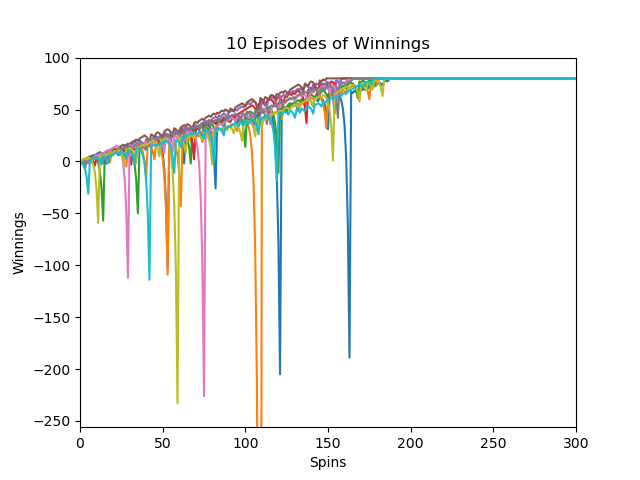
\includegraphics[height=5.5cm]{figure_1.png} & 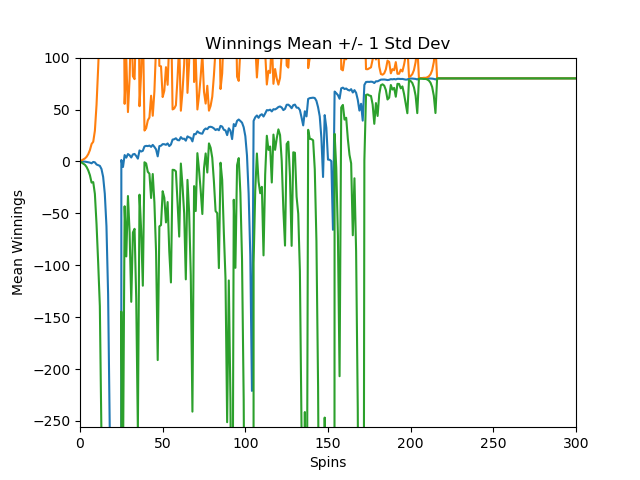
\includegraphics[height=5.5cm]{figure_2.png} \\
		\textbf{Figure 1} & \textbf{Figure 2} \\
		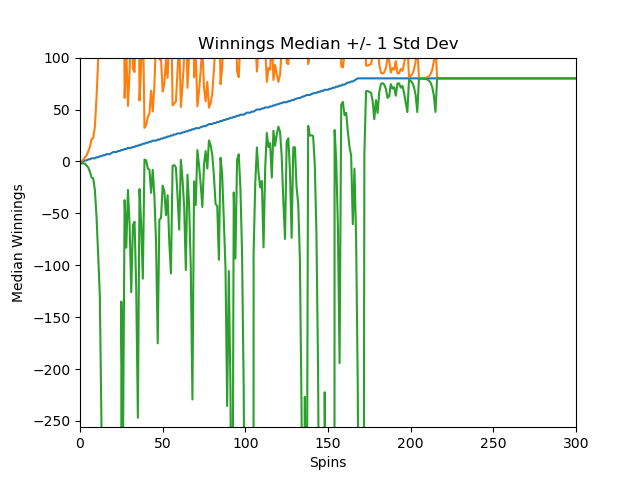
\includegraphics[height=5.5cm]{figure_3.png} & \\
		\textbf{Figure 3} & \\
	\end{tabular}
\end{figure}


\subsection{Question 1}
In Experiment 1, based on the experiment results calculate and provide the estimated probability of winning \$80 within 1000 sequential bets. Thoroughly explain your reasoning for the answer using the experiment output. Your explanation should NOT be based on estimates from visually inspecting your plots. 

The estimated probability of winning \$80 within 1000 sequential bets can be calculated by taking a total count of all \$80 winnings on the last spin (100th) and dividing it by the total number of episodes. The estimated probability is 100\%, all 1000 episodes in experiment 1 had earned \$80 in winnings by the last spin.


\subsection{Question 2}
In Experiment 1, what is the estimated expected value of winnings after 1000 sequential bets? Thoroughly explain your reasoning for the answer

The expected value of winnings for experiment 1 was \$80.  All 1000 episodes had won \$80 by the time of the last spin.


\subsection{Question 3}
 In Experiment 1, do the upper standard deviation line (mean + stdev) and lower standard deviation line (mean – stdev) reach a maximum (or minimum) value and then stabilize? Do the standard deviation lines converge as the number of sequential bets increases? Thoroughly explain why it does or does not. 
 
 The upper and lower standard deviation lines converge on the mean on the 215th spin. This is when the mean winnings reaches \$80.  Since we stop betting once \$80 is reached and carry the number forward until the 1000th spin, the mean stops changing and the standard deviation drops to 0.  If a stopping point of \$80 in winnings did not exist, the upper and lower standard deviation lines would not have converged at all.


\section{Experiment 2}

\begin{figure}[h]
	\begin{tabular}{cc}
		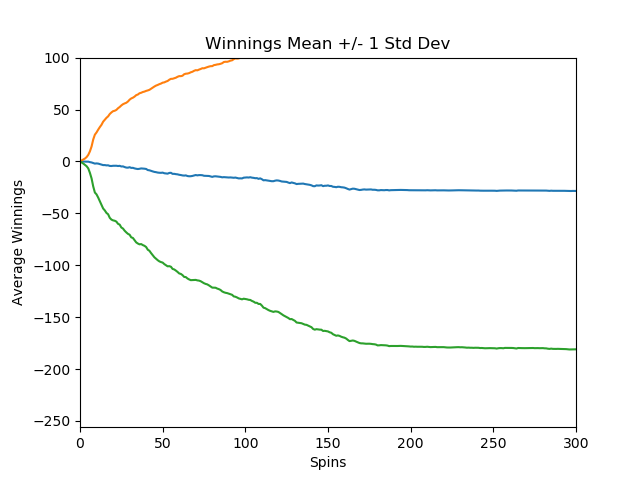
\includegraphics[height=5.5cm]{figure_4.png} & 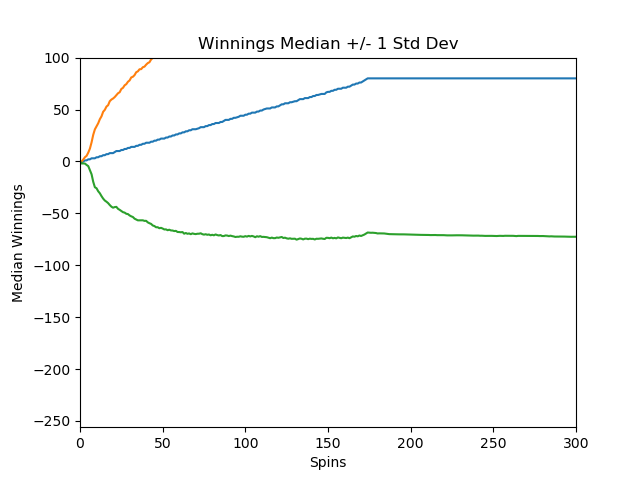
\includegraphics[height=5.5cm]{figure_5.png} \\
		\textbf{Figure 4} & \textbf{Figure 5} \\
	\end{tabular}
\end{figure}


\subsection{Question 4}
In Experiment 2, based on the experiment results calculate and provide the estimated probability of winning \$80 within 1000 sequential bets. Thoroughly explain your reasoning for the answer using the experiment output. Your explanation should NOT be based on estimates from visually inspecting your plots. 

The probability of winning \$80 in experiment 2 is 0.668, and can be calculated using the same method used in experiment 1. The answer is different in this case because we no longer have an unlimited bank roll, and must only bet what we have available in the current model.

\subsection{Question 5}
In Experiment 2, what is the estimated expected value of winnings after 1000 sequential bets? Thoroughly explain your reasoning for the answer. 

The expected value for experiment 2 is -\$31.552.  This is the mean of all winnings on the 1000th spin.  You can expect to lose \$31.55 on average when the bettor is limited to \$256 in losses as per the experiment.  The probability of winning by betting on one color is approximately 0.47368, so the bettor will lose more times than win.

\subsection{Question 6}
In Experiment 2, do the upper standard deviation line (mean + stdev) and lower standard deviation line (mean – stdev) reach a maximum (or minimum) value and then stabilize? Do the standard deviation lines converge as the number of sequential bets increases? Thoroughly explain why it does or does not. 

The upper and lower standard deviation lines stabilize as the mean winnings approach the estimated expected value. As the mean starts stabilizing around the estimated expected value, the standard deviation also starts stabilizing.
The upper standard deviation line reaches its max on the 848th spin, while the lower standard deviation lines reaches its minimum on the 867th spin. The mean winnings on these spins is -\$31.34 and -\$31.64 respectively.

\section{Summary}

\subsection{Question 7}
What are some of the benefits of using expected values when conducting experiments instead of simply using the result of one specific random episode? 

The benefits of using expected values is from the law of large numbers or central limit theorem.  As the number of trials grows the average of the results obtained grows closer to the expected value, allowing the average of the trials to be used as an estimate of the expected value.

\vspace{30mm}
\textit{Recommendation: If the upper and lower standard deviation lines do not converge and/or stabilize, explain why they do not. If they converge and/or stabilize, also discuss the value(s) at which they do so.} 
\end{document}